%%%%%%%%%%%%%%%%%%%%%%%%%%%%%%%%%%%%%%%%%%%%%%%%%%%%%%%%%%%%%%%%%
% Contents : The transactions chapter
% $Id : grisbi-manuel-transactions.tex,v 0.4 2002/10/27 Daniel Cartron
% $Id : grisbi-manuel-transactions.tex, v 0.5.0 2004/06/01 Loic Breilloux
% some of its content was in tips chapter  : 
% $Id : grisbi-manuel-tips.tex, v 0.4 2002/10/27 Daniel Cartron
% $Id : grisbi-manuel-transactions.tex, v 0.6.0 2011/11/17 Jean-Luc Duflot
% some of its content was in tips chapter :
% $Id : grisbi-manuel-tips.tex, v 0.5.0 2004/06/01 Loic Breilloux
% $Id : grisbi-manuel-transactions.tex, v 0.8.9 2012/04/27 Jean-Luc Duflot
% $Id : grisbi-manuel-transactions.tex, v 1.0 2014/02/12 Jean-Luc Duflot
% some of its content was in accounts chapter :
% $Id : grisbi-manuel-accounts.tex, v 0.8.9 2012/04/27 Jean-Luc Duflot
%%%%%%%%%%%%%%%%%%%%%%%%%%%%%%%%%%%%%%%%%%%%%%%%%%%%%%%%%%%%%%%%%

\chapter{Opérations d'un compte\label{transactions}}

Les différents comptes que vous avez créés contiennent les opérations. Pour afficher la liste des comptes enregistrés dans votre fichier de comptes, utilisez la barre d'information ou le panneau de navigation (voir le chapitre \vref{home}, \menu{Accueil} et la section \vref{accounts-list}, \menu{Liste des comptes}).

Pour afficher les opérations d'un compte, sélectionnez ce compte dans la liste : l'onglet \menu{Opérations} s'affiche par défaut. Il possède quatre éléments principaux :

\begin{itemize}
	 \item la barre d'outils ;
	 \item la liste des opérations ;
	 \item le formulaire de saisie des opérations ;
	 \item le \indexword{solde pointé}\index{solde !pointé}.
\end{itemize}

% espace avant Attention ou Note  : 5 mm
\vspacepdf{5mm}
\textbf{Note} : si vous n'avez jamais fait de rapprochement, donc pas de pointages, Grisbi ne peut ni calculer ni afficher de solde pointé.


\section{Barre d'outils\label{transactions-functions}}


La barre d'outils présente les fonctions suivantes  : 

\begin{itemize}
	 \item \menu{Nouvelle Opération} : va à la fin de la liste des opérations et ouvre le formulaire de saisie vierge ;
	 \item \menu{Supprimer} : supprime l'opération sélectionnée ;
	 \item \menu{Éditer} : ouvre le formulaire de saisie pour l'opération sélectionnée et permet de la modifier ;
	 \item \menu{Rapprocher} : ouvre la page de rapprochement du compte sélectionné (voir le chapitre \vref{reconciliation}, \menu{Rapprochement bancaire}) ;
	 \item \menu{Imprimer} : ouvre la fenêtre de sélection de l'imprimante et de ses
	options ;
	 \item \menu{Affichage} : ouvre un menu déroulant ; vous pouvez choisir l'\indexword{affichage des opérations}\index{affichage !opérations} parmi quatre possibilités (\menu{Vue simple}, \menu{Mode \og deux lignes \fg{}}, \menu{Mode \og trois lignes \fg{}} et \menu{Vue complète}), ainsi que l'affichage ou non des \indexword{opérations rapprochées}\index{affichage !opérations rapprochées} et des \indexword{lignes d'archives}\index{affichage !lignes d'archives}.
\end{itemize}

% espace pour changement de thème
\vspacepdf{5mm}
Les options du menu \menu{Affichage} influent par défaut sur l'affichage de tous les comptes. Vous pouvez préférer un affichage différent pour chaque compte, cela est configurable dans le menu \menu{Édition - Préférences}  (voir le paragraphe \vref{setup-operations-list-differenciation}, \menu{Différenciation des comptes}).
 
La \indexword{barre d'outils}\index{barre d'outils !déplacement} peut être déplacée dans l'écran en cliquant sur sa poignée (petit rectangle vertical à gauche de la barre) et en la déplaçant. Pour la réattacher à son emplacement d'origine dans le pavé des détails, la remettre en haut de la fenêtre, le haut de la poignée sur le petit trait qui visualise sa place d'origine.


\section{Liste des opérations\label{transactions-list}}


\subsection{Description\label{transactions-list-description}}

La liste des opérations s'affiche dans le panneau des \ifIllustration détails\refimage{transactions-list-img}.
\else détails.
\fi

\ifIllustration 
% image centrée 
\begin{figure}[ht]
\begin{center}
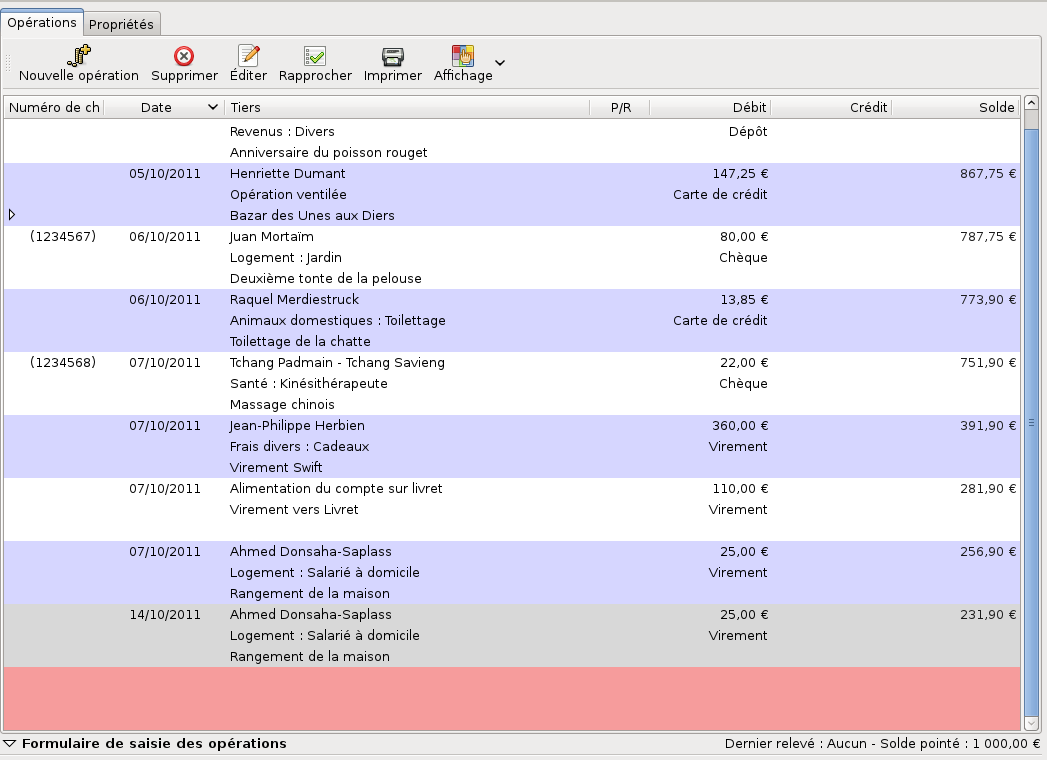
\includegraphics[scale=0.5]{image/screenshot/transactions_list}
\end{center}
\caption{Liste des opérations}
\label{transactions-list-img}
\end{figure}
% image centrée 
\fi

Elle affiche en haut la barre des libellés des colonnes. Vous pouvez \indexword{élargir ou rétrécir une colonne}\index{colonne !largeur} en cliquant sur le séparateur entre deux colonnes et en le déplaçant. Pour rétablir la largeur des colonnes à leur valeur par défaut, sélectionnez le menu \menu{Affichage - Réinitialiser la largeur des colonnes}.

Vous pouvez déplacer la liste des opérations vers le haut ou vers le bas avec la molette de la souris, ou bien avec la souris et l'ascenseur vertical. Le déplacement vers la gauche ou la droite se fait avec la souris et l'ascenseur horizontal.

Vous pouvez choisir d'afficher ou non les \indexword{opérations rapprochées}\index{affichage !opérations rapprochées} et les \indexword{lignes d'archives}\index{affichage !lignes d'archives} : sélectionnez \menu{Affichage - Montrer les opérations rapprochées} ou \menu{Affichage - Montrer les lignes d'archives} dans la barre de menus ou dans la barre d'outils (voir la section \vref{home-menus-display}, \menu{Menu Affichage} ou la fonction \menu{Affichage} dans la section \vref{transactions-functions}, \menu{Barre d'outils}).

% espace pour changement de thème
\vspacepdf{5mm}
Du point de vue de la base de données de Grisbi, une opération est constituée de ses \indexword{champs d'information}\index{champ d'information !définition}. Les champs d'information de chaque opération s'affichent dans les différentes \indexword{cellules}\index{cellule !champ d'information} définies par l'intersection des lignes et des colonnes. Il ne peut y avoir au  maximum que quatre lignes et sept colonnes, ce qui définit un maximum de vingt-huit champs d'information pour chaque opération.

Chaque opération peut être affichée sur 1, 2, 3 ou 4 lignes, suivant le mode d'affichage sélectionné (voir la section \vref{home-menus-display}, menu \menu{Affichage} dans la barre de menus ou la fonction \menu{Affichage} dans la section \vref{transactions-functions}, \menu{Barre d'outils}). L'affichage courant y est indiqué par une coche. 

Vous pouvez aussi configurer le contenu de ces lignes, ainsi que la mémorisation des réglages de l'affichage, individuellement pour chaque compte, dans le menu \menu{Édition - Préférences} (voir les sections \vref{setup-operations-list}, \menu{Comportement de la liste} et \vref{setup-operations-cells}, \menu{Cellules de la liste des opérations}).

Le \indexword{libellé d'une colonne}\index{colonne !libellé} est toujours le nom du champ d'information  affiché dans la première ligne des opérations.

Pour des raisons de lisibilité de l'affichage, Grisbi n'affiche aucune bordure aux cellules, colonnes, lignes et opérations, mais présente une alternance de couleurs de fond violet et blanc{\couleurs} à chaque ligne.


\subsection{Champs d'information et de saisie\label{transactions-list-fields}}

Grisbi sait gérer, pour chaque opération, une liste complète de champs d'information et de saisie\index{champs d'information}\index{champs de saisie}, qui sont les suivants :

\begin{itemize}
	\item \menu{Date de l'opération}\index{date !opération} : \indexword{date} à laquelle est réalisée l'opération ; elle peut être utilisée pour calculer les soldes ;
	\item \menu{Date de valeur}\index{date !valeur} : \indexword{date} à laquelle la banque comptabilise l'opération ; c'est cette date qui fait foi pour le calcul des intérêts et des agios ; elle peut être utilisée pour calculer les soldes ;
	\item \menu{Tiers} ;
	\item \menu{Imputation budgétaire} ;
	\item \menu{Débit} : montant débité du solde du compte ; dans le cas d'opérations dans une \indexword{devise différente}\index{devise !différente} de celle du compte, montant de l'opération dans la devise différente ;
	\item \menu{Crédit} ;
	\item \menu{Solde} : montant toujours calculé \emph{après} l'opération affichée sur la même ligne ; il dépend chronologiquement du \indexword{tri primaire}\index{tri !primaire} sélectionné ; un \indexword{solde négatif}\index{solde !négatif} est affiché en rouge{\couleur} ;
	\item \menu{Montant} : dans le cas d'opérations dans une \indexword{devise différente}\index{devise !différente} de celle du compte, montant de l'opération dans la devise du compte ;
	\item \menu{Moyen de paiement} ;
	\item \menu{\No rapprochement} : numéro de chaque rapprochement dans chaque compte ;
	\item \menu{Exercice} ;
	\item \menu{Catégorie} ;
	\item \menu{P/R} : statut de l'opération, \emph{Pointé} ou \emph{Rapproché} ;
	\item \menu{Pièce comptable}, par exemple le numéro de la facture (\menu{Pièce comptable} et \menu{Numéro d'opération} sont des références réciproques qui assurent la traçabilité de l'opération) ;
	\item \menu{Remarques} : informations éventuelles sur l'opération ;
	\item \menu{Infos banque/guichet}, utile uniquement si vous enregistrez un chèque reçu ;
	\item \menu{Numéro d'opération} : il s'agit d'un numéro d'ordre unique que Grisbi attribue à chaque opération ; vous pouvez reporter ce numéro sur la pièce comptable correspondante (\menu{Numéro d'opération} et \menu{Pièce comptable} sont des références réciproques qui assurent la traçabilité de l'opération) ;
	\item \menu{\No chèque} ou \menu{\No chèque/virement }, si le mode de règlement sélectionné permet cette saisie ;
	\item \menu{Devise de l'opération} ;
	\item \menu{Taux de change} ;
	\item \menu{Mode de règlement de la \indexword{contre-opération}}\index{contre-opération} : vous pouvez le configurer pour chaque compte dans le menu \menu{Édition - Préférences} (voir la section \vref{setup-resources-modes}, \menu{Modes de règlement}) ;
	\item \menu{Auto/Manuel} : statut de l'exécution d'une opération planifiée
\end{itemize}

% espace pour changement de thème
\vspacepdf{5mm}
La liste des opérations et le formulaire de saisie utilisent chacun un sous-ensemble de ces champs. Vous pouvez voir les deux listes complètes dans les tableaux du menu \menu{Édition - Préférences}, onglets \menu{Cellules de la liste des opérations} et \menu{Contenu}, ou dans les sections \vref{setup-operations-cells}, \menu{Cellules de la liste des opérations} et \vref{setup-form-content}, \menu{Contenu}.


\subsection{Gestion des champs d'information\label{transactions-list-fields-manage}}

Grisbi affiche par défaut, dans la liste des opérations, un certain nombre de ces champs (tiers, catégorie, débit, etc.). Mais vous pouvez aussi \indexword{gérer les champs d'information}\index{champ d'information !gestion} différemment, c'est à  dire afficher de nouveaux champs, les modifier ou en supprimer l'affichage, à votre convenance. 
Vous pouvez soit faire ces manipulations dans le menu \menu{Édition - Préférences - Opérations - Cellules de la liste des opérations}, qui offre un aperçu complet de la disposition des champs dans les cellules, et permet de faire plusieurs modifications facilement (voir la section \vref{setup-operations-cells}, \menu{Cellules de la liste des opérations}), soit le faire directement dans la liste des opérations, en suivant les méthodes ci-dessous :


\subsubsection{Ajout d'un champ d'information\label{transactions-list-fields-add}}

Pour \indexword{ajouter un champ d'information}\index{champ d'information !ajouter} dans une cellule, procédez comme suit :

\begin{enumerate}
	 \item sélectionnez \menu{Affichage - Vue complète} dans la barre d'outils ou \menu{Affichage - Montrer quatre lignes par opération} dans la barre de menus, pour vous assurer de voir toutes les vingt-huit cellules ;
	 \item cliquez-droit dans une des cellules vides de la colonne où vous voulez ajouter ce champ : faites-le précisément, car rien ne permet d'identifier sur quelle cellule vous avez cliqué ;
	 \item  un menu contextuel s'affiche ; sélectionnez \menu{Modifier le contenu de la cellule} ; vérifiez qu'il n'y a pas déjà de champ d'information dans cette cellule, en constatant qu'aucun champ de la liste déroulante n'a de coche à gauche de son nom ;
	 \item choisissez un champ d'information proposé dans la liste ; ce champ s'ajoute dans la cellule choisie, et toutes les opérations de la liste l'affichent.
\end{enumerate}


\subsubsection{Modification d'un champ d'information\label{transactions-list-fields-modify}}

Pour \indexword{modifier un champ d'information}\index{champ d'information !modifier} dans une cellule, procédez comme suit :

\begin{enumerate}
	 \item sélectionnez \menu{Affichage - Vue complète} dans la barre d'outils ou \menu{Affichage - Montrer quatre lignes par opération} dans la barre de menus, pour vous assurer de voir toutes les vingt-huit cellules ;
	 \item cliquez-droit dans une des cellules de la colonne dont vous voulez modifier le champ : faites-le précisément, car rien ne permet d'identifier sur quelle cellule vous avez cliqué ;
	 \item  un menu contextuel s'affiche ; sélectionnez \menu{Modifier le contenu de la cellule} ; le champ d'information actuel dans cette cellule est indiqué par une coche à gauche de son nom ;
	 \item choisissez un autre champ d'information proposé dans la liste ; ce champ remplace le précédent dans la cellule choisie, et toutes les opérations de la liste l'affichent.
\end{enumerate}


\subsubsection{Suppression d'un champ d'information\label{transactions-list-fields-remove}}

Pour \indexword{supprimer un champ d'information}\index{champ d'information !supprimer} dans une cellule, procédez comme suit :

\begin{enumerate}
	 \item sélectionnez \menu{Affichage - Vue complète} dans la barre d'outils ou \menu{Affichage - Montrer quatre lignes par opération} dans la barre de menus, pour vous assurer de voir toutes les vingt-huit cellules ;
	 \item cliquez-droit dans la cellule du champ à supprimer : faites-le précisément, car rien ne permet d'identifier sur quelle cellule vous avez cliqué ;
	 \item un menu contextuel s'affiche ; sélectionnez \menu{Modifier le contenu de la cellule} ; le champ d'information actuel dans cette cellule est indiqué par une coche à gauche de son nom ;
	 \item choisissez \menu{Effacer la cellule} dans la liste ; le champ d'information actuel disparaît pour toutes les opérations de la liste (mais les informations ne sont en aucun cas supprimées de votre fichier de comptes).
\end{enumerate}

\subsubsection{Déplacement d'un champ d'information\label{transactions-list-fields-move}}

Pour \indexword{déplacer un champ d'information}\index{champ d'information !déplacer}, vous pouvez le supprimer puis l'ajouter dans un autre champ vide, mais vous pouvez aussi le faire dans le menu \menu{Édition - Préférences - Opérations - Cellules de la liste des opérations}. Voir la section \vref{setup-operations-cells}, \menu{Cellules de la liste des opérations}.


\subsection{Tris\label{transactions-list-sorts}}

Pour changer l'ordre d'affichage des opérations, vous pouvez faire un \indexword{tri sur les opérations}\index{tri !opérations} sur un des champs d'information ; procédez comme suit :

\begin{enumerate}
	  \item cliquez-droit sur le libellé de la colonne qui contient le champ d'information choisi comme critère de \gls{tri} ;
	  \item un menu contextuel affiche la liste des champs de cette colonne ; 	sélectionnez le champ choisi comme critère de tri ;
	  \item toutes les opérations s'affichent, triées selon le critère choisi ;
	  \item un petit triangle noir apparaît à droite du libellé de la colonne ; il pointe vers le bas si le tri est ascendant, vers le haut si le tri est descendant ;
% saut de ligne pour indentation correcte de la note dans la liste

	  \textbf{Note} : ces triangles peuvent être remplacés, en fonction du thème de l'environnement de bureau ou du gestionnaire de fenêtres que vous utilisez, par d'autres caractères tels que +, -, >, <, etc.
	  \item cliquez sur ce triangle pour changer l'ordre du tri.
\end{enumerate}

\textbf{Note} : un tri sur l'affichage réalisé ainsi n'affecte en aucun cas le solde à chaque ligne, qui est calculé après chaque opération ; suivant le tri et les options d'affichage que vous avez choisi, le solde à chaque ligne peut présenter une évolution non chronologique. 

%espace pour changement de thème
\vspacepdf{5mm}
Vous pouvez aussi configurer l'ordre général des tris dans le menu \menu{Édition - Préférences} (voir la section \vref{setup-operations-list-modes}, \menu{Modes d'affichage}).

\textbf{Note} : le choix du critère de \gls{tri primaire} (date d'opération ou date de valeur) qui peut y avoir été fait modifie nécessairement le solde affiché à chaque ligne d'opération, puisque Grisbi calcule et affiche le solde à chaque ligne.


\section{Formulaire de saisie\label{transactions-form}}


Le formulaire de saisie est situé en-dessous de la liste des opérations, où une ligne affiche, à gauche de \menu{Formulaire de saisie des opérations}, un petit triangle qui  permet d'\indexword{afficher ou de masquer}\index{formulaire de saisie !masquer-afficher} \ifIllustration ce formulaire\refimage{transactions-form-img}.
\else ce formulaire.
\fi

\ifIllustration
% image centrée 
\begin{figure}[htbp]
\begin{center}
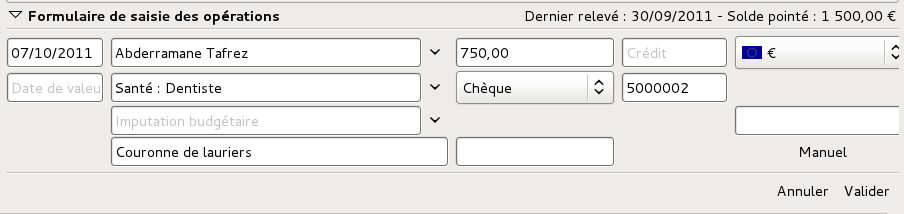
\includegraphics[scale=0.5]{image/screenshot/transactions_form}
\end{center}
\caption{Formulaire de saisie des opérations}
\label{transactions-form-img}
\end{figure}
% image centrée 
\fi

\textbf{Note} : ce triangle peut être remplacé, en fonction du thème de l'environnement de bureau ou du gestionnaire de fenêtres que vous utilisez, par d'autres caractères tels que +, -, >, <, etc.

Le formulaire de saisie comprend par défaut les sept champs suivants : \menu{Date de l'opération}, \menu{Tiers}, \menu{Débit}, \menu{Crédit}, \menu{Catégorie}, \menu{Moyen de paiement} et \menu{Remarques}. Vous pouvez avoir besoin de champs supplémentaires, par exemple \menu{Exercice}, \menu{Imputation budgétaire} ou autre. Pour cela, allez dans le menu \menu{Édition - Préférences - Formulaire des opérations - Contenu}, ou cliquez-droit dans le formulaire de saisie, dans une zone grise en dehors des champs de saisie, sélectionnez \menu{Configurer le formulaire} (voir la section \vref{setup-form}, \menu{Formulaire des opérations}).

%espace pour changement de thème
\vspacepdf{5mm}
Pour connaître l'ensemble des champs que peut gérer Grisbi, voir la section \vref{transactions-list-fields}, \menu{Champs d'information et de saisie}.

Une fois le formulaire affiché, un menu contextuel accessible par un clic-droit dans un champ de saisie permet d'effectuer les actions suivantes :

\begin{itemize}
	 \item \menu{Couper} (la sélection) ;
	 \item \menu{Copier} (la sélection) ;
	 \item \menu{Coller} (la sélection) ;
	 \item \menu{Supprimer} (la sélection) ;
	 \item \menu{Tout sélectionner} (dans le champ de saisie) ;
	 \item \menu{Méthodes de saisie}\index{méthodes de saisie} ;
	 \item \menu{Insérer un caractère de contrôle Unicode}\index{caractère de contrôle Unicode}.
\end{itemize}

%espace pour changement de thème
\vspacepdf{5mm}
Le choix \menu{\gls{methodes de saisie}} permet de changer les caractères accentués.

Le choix \menu{Insérer un \gls{caractere de controle Unicode}} permet d'insérer un code Unichar qui modifie la présentation ; par exemple RLO (forçage droite-à-gauche) renverse l'ordre des lettres et la position du texte.

De plus, un autre menu contextuel, accessible par un clic-droit en dehors d'un champ de saisie, permet d'accéder à la \indexword{configuration du formulaire}\index{formulaire de saisie !configuration} : vous pouvez en configurer précisément le contenu, la présentation, le comportement, ainsi que les paramètres d'aide à la saisie, dans le menu \menu{Édition - Préférences} (voir la section \vref{setup-form}, \menu{Formulaire des opérations}).


\section{Solde pointé\label{transactions-balance}}


En-dessous de la liste des opérations, sur la même ligne que le formulaire de saisie, s'affichent à droite deux informations  : la date du dernier relevé bancaire rapproché et le \indexword{solde pointé}\index{solde !pointé} correspondant à ce dernier rapprochement, à moins que vous ne pointiez très régulièrement vos opérations, auquel cas il correspond au solde tel que le connaît votre banque (voir le chapitre \vref{reconciliation}, \menu{Rapprochement bancaire}).

\ifIllustration
% saut de page pour titre solidaire
\newpage
\else
\fi


\section{Sélection d'une opération \label{transactions-selection}}


Pour sélectionner une opération, vous avez deux moyens :

\begin{itemize}
	 \item cliquez sur une de ses lignes ;
	 \item déplacez la sélection avec les touches du clavier \key{Flèche Haut} et \key{Flèche Bas}.
\end{itemize}

L'opération apparaît alors sur fond rouge{\couleur} et ses détails s'affichent dans le formulaire.

% espace pour changement de thème
\vspacepdf{5mm}
Un menu contextuel est disponible sur la liste des opérations. Un clic-droit sur la ligne d'une opération permet les fonctions suivantes, selon le contexte :
% espace avant image 5mm
\vspacepdf{3mm}

\begin{itemize}
	\ifIllustration
	% image entourée par une liste (picins)
	% Pas de référence à l'illustration car erreur de numéro de figure avec picins
	%supprimé car en html les figures entourées ne sont pas numérotées, et la numérotation des figures centrées décalée par rapport au pdf
	%\piccaption{Menu contextuel de la liste des opérations}
	\label{transactions-contextMenu-img}
	\parpic[r]{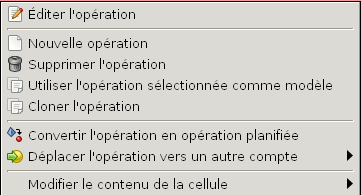
\includegraphics[scale=0.50]{image/screenshot/transactions_contextMenu}}
	% image entourée par une liste (picins)
	\fi
	 \item \menu{Afficher la contre-opération}\index{contre-opération !afficher} : ce choix est présent seulement si l'opération est un virement ;
	 \item \menu{Éditer l'opération} ;
	 \item \menu{Nouvelle opération} ;
	 \item \menu{Supprimer l'opération} ;
	 \item \menu{Utiliser l'opération sélectionnée comme modèle} ;
	 \item \menu{Cloner l'opération} ;
	 \item \menu{Convertir l'opération en opération planifiée} : cela permet de créer
	facilement des échéances après coup ;
	 \item \menu{Déplacer l'opération vers un autre compte} ;
	 \item \menu{Modifier le contenu de la cellule}.
\end{itemize}


\section{Saisie d'une nouvelle opération\label{transactions-new}}


La saisie d'une opération se fait dans le formulaire de saisie, situé en-dessous de la liste des opérations.

Pour saisir une nouvelle opération, ouvrez ou affichez le formulaire de saisie avec l'une de ces méthodes :

\begin{itemize}
	 \item sélectionnez la ligne vide en bas de la liste des opérations et appuyez sur la touche \key{Entrée} ;
	 \item appuyez sur la combinaison de touches \key{Ctrl}\key{T} ;
	 \item double-cliquez sur la ligne vide ;
	 \item dans la barre de menus, sélectionnez \menu{Édition - Nouvelle opération} ;
	 \item dans la barre de menus, sélectionnez \menu{Montrer le formulaire de saisie d'opérations} ;
	 \item dans la barre d'outils, cliquez sur \menu{Nouvelle opération} ;
	 \item dans le menu contextuel, sélectionnez \menu{Nouvelle opération} ;
	 \item cliquez sur le petit triangle d'\indexword{affichage/masquage}\index{formulaire de saisie !masquer-afficher} du formulaire de saisie des opérations à gauche de son libellé.
% saut de ligne pour indentation correcte de la note dans la liste

	 \textbf{Note} : ce triangle peut être remplacé, en fonction du thème de l'environnement de bureau ou du gestionnaire de fenêtres que vous utilisez, par d'autres caractères tels que +, -, >, <, etc.
\end{itemize}

% espace après Attention ou Note  : 5 mm
\vspacepdf{5mm}
La dernière ligne, entièrement vide, en bas de la liste des opérations, apparaît sur fond rouge{\couleur}, le formulaire de saisie vierge s'affiche, avec seule la date du jour, ou la dernière date entrée, sur fond bleu{\couleur}.

% espace pour changement de thème
\vspacepdf{5mm}
Saisissez les différentes informations concernant votre opération dans les différents champs du formulaire. Certains champs peuvent être renseignés soit avec le clavier, soit avec une liste déroulante. Si vous utilisez le clavier, cette saisie sera automatiquement enregistrée dans la liste déroulante de ce champ. Si vous le voulez, vous pourrez toujours supprimer plus tard ce choix dans la liste : reportez-vous aux différents chapitres traitant de ces listes (\menu{Tiers}, \menu{Catégories}, \menu{Imputations budgétaires} et les différents onglets de la section \menu{Ressources} du menu \menu{Édition - Préférences}.

Chaque champ de saisie doit être renseigné par le type de  donnée qui lui convient (date, nombre, texte), sinon l'arrière-plan du champ deviendra rouge{\couleur}. 

Une fois le dernier champ du formulaire saisi et validé, l'opération s'affiche dans la liste des opérations, et la ligne active, en rouge{\couleur}, passe à la dernière ligne vide de la liste.

% espace pour changement de thème
\vspacepdf{5mm}
Les sous-sections suivantes donnent les différentes méthodes de saisie disponibles.


\subsection{Commandes principales au clavier\label{transactions-new-keyboard}}

La touche \key{Tabulation} permet le déplacement dans le formulaire.

La touche \key{Entrée} permet soit de se déplacer dans le formulaire de saisie, soit de valider la saisie ; cela est configurable dans le menu \menu{Édition - Préférences} (voir la section \vref{setup-form-behaviour}, \menu{Comportement}). Cette  configuration affecte à la fois la touche \key{Entrée} du clavier alphabétique et celle du pavé numérique.

La touche \key{Échap} permet d'annuler la saisie en cours.


\subsection{Saisie de date au clavier\label{transactions-new-dates}}

La date du jour ou la dernière date entrée s'affiche automatiquement à l'ouverture du formulaire.

%espace pour changement de thème
\vspacepdf{5mm}
Vous pouvez saisir la date avec l'un de ces formats :

\begin{itemize}
	 \item jj/mm/aa (avec délimiteur) ;
	 \item jjmmaa ou jjmm (sans délimiteur) ; dans ce cas, vous devrez bien utiliser deux chiffres pour les jour, mois et année ;
	 \item j/m/a si le jour, le mois ou l'année ne comportent qu'un seul chiffre (par ex. : 1/1/1 pour le premier janvier 2001).
\end{itemize}

De plus, il n'est pas nécessaire de saisir l'année si celle-ci est identique à l'année en cours, ni le mois si celui-ci est le mois en cours, car Grisbi complétera automatiquement.

%espace pour changement de thème
\vspacepdf{5mm}
Enfin, vous pouvez incrémenter ou décrémenter la date affichée :

\begin{itemize}
	 \item par jour avec les touches \key{+} ou \key{-} ;
	 \item par semaine avec les touches \key{Majuscule} \key{+} ou \key{Majuscule} \key{-} ;
	 \item par mois avec les touches\key{Page Haut} ou \key{Page Bas} ;
	 \item par année avec les combinaisons de touches \key{Majuscule} \key{Page Haut}
	ou \key{Majuscule} \key{Page Bas}.
\end{itemize}


\subsection{Saisie de date au calendrier\label{transactions-new-calendar}}

Un double-clic sur la date, ou la combinaison de touches \key{Ctrl} \key{Entrée}, affiche un calendrier permettant de sélectionner la date.

%espace pour changement de thème
\vspacepdf{5mm}
Vous pouvez alors sélectionner une nouvelle date avec la souris ou le clavier :
% espace avant image 5mm
\vspacepdf{3mm}
\begin{itemize}
	% image entourée par une liste ( picins)
	% Pas de référence à l'illustration car erreur de numéro de figure avec picins.
	\ifIllustration
	% supprimé car en html les figures entourées ne sont pas numérotées, et la numérotation des figures centrées décalée par rapport au pdf
	%\piccaption{Calendrier de sélection de date}
	\label{transactions-calendar-img}
	\parpic[r]{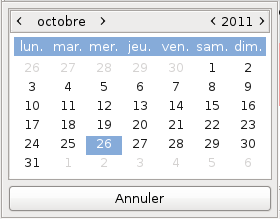
\includegraphics[scale=0.5]{image/screenshot/transactions_calendar}}
	% image entourée par une liste ( picins)
	\fi
	\item les touches \key{+} ou \key{-}, de même que \key{Flèche Gauche} ou \key{Flèche Droite}, permettent de passer au jour précédent ou suivant ;
	\item les touches \key{Flèche Haut} ou \key{Flèche Bas} permettent de passer à la semaine précédente ou suivante ;
	\item les touches \key{Page Haut} ou \key{Page Bas} permettent de passer au mois précédent ou suivant ;
	\item les touches \key{Début} ou \key{Fin} permettent de passer au premier jour ou au dernier jour du mois.
	\item un clic sur le bouton \menu{Annuler} ou l'appui sur la touche \key{Échap} ferme le calendrier sans modifier la date ;
	\item un double-clic ou l'appui sur la touche \key{Entrée} valide la date sélectionnée.
\end{itemize}

\ifIllustration
% espace après image entourée
\vspacehevea{3mm}
\else
\fi


\subsection{Listes déroulantes\label{transactions-new-lists}}

Certains champs disposent d'une liste déroulante de choix déjà définis. Vous pouvez y sélectionner un libellé avec la souris, ou préférer saisir les données au clavier dans le champ de saisie.

L'ouverture d'une liste déroulante peut se faire avec la souris en cliquant sur le petit triangle à droite du champ, ou avec les touches du clavier \key{Page Bas} ou \key{Flèche bas}, le déplacement dans cette liste peut se faire avec la souris, ou avec les touches \key{Page Haut}, \key{Page Bas}, \key{Flèche haut} ou \key{Flèche bas}, et la validation d'un choix à l'intérieur d'une liste déroulante se fait avec la touche \key{Entrée}.

\textbf{Note} : ces triangles peuvent être remplacés, en fonction du thème de l'environnement de bureau ou du gestionnaire de fenêtres que vous utilisez, par d'autres caractères tels que +, -, >, <, etc.

%espace pour changement de thème
\vspacepdf{5mm}
Grisbi vous proposera de compléter automatiquement le mot saisi dès qu'il en aura reconnu suffisamment de caractères. L'\indexword{auto-complètement}\index{champ de saisie !auto-complètement} apparaît sur fond bleu{\couleur}. Pour accepter celui proposé, appuyez sur la touche \key{Tabulation} ou la touche \key{Entrée}, selon votre choix de configuration, sinon continuez la saisie.

Les listes déroulantes des devises, exercices et modes de règlement s'ouvrent avec la touche \key{Espace} ; on s'y déplace  avec les touches \key{Flèche Haut} et \key{Flèche Bas} et l'on  valide avec la touche \key{Espace}.


\subsection{Saisie de formules\label{transactions-new-numbers}}

Dans le formulaire de saisie, vous pouvez saisir les nombres, avec ou sans décimales, dans les champs tels que \menu{Débit} et \menu{Crédit}, à l'aide du clavier.

Vous pouvez aussi y saisir des \indexword{formules arithmétiques}\index{champ de saisie !formule arithmétique}\index{formule arithmétique !champ de saisie} simples, à l'aide des quatre opérateurs d'addition, soustraction, multiplication et division. Cela remplace la \indexword{calculatrice}\index{calculatrice} sur votre bureau.

Pour saisir une formule, saisissez-la comme si c'était un texte, par exemple \og 3,40-2,10\fg{} , puis continuez normalement la saisie des autres champs de votre opération ; si elle est mal écrite, elle s'affiche sur fond rouge{\couleur}. Lorsque vous la validez, le résultat \og 1,30 \fg{} s'affiche dans le champ de saisie, et si la formule est toujours mal écrite, le message \og \#\#\#ERR\#\#\# \fg{} s'affiche à la place et sur fond rouge{\couleur}.

Cette calculatrice accepte la multiplication ou la division, mais de manière exclusive de l'addition ou de la soustraction ; c'est-à-dire qu'on peut mélanger additions et soustractions dans une saisie mais pas une multiplication (ou une division) et un quelconque autre opérateur : on ne peut pas mettre de parenthèses pour indiquer un ordre de priorité d'opération.

Cette fonctionnalité peut être très utile, notamment pour réajuster les montants d'une opération ventilée en cas d'écart. 


\subsection{Remise de chèques ou d'espèces\label{transactions-new-cheque}}

Pour enregistrer une \indexword{remise de chèques}\index{remise !chèques}, vous les déposez d'abord sur votre compte bancaire à la banque qui vous remet un bordereau de remise, puis vous saisissez l'opération de remise, en crédit sur votre compte bancaire.

Pour enregistrer une \indexword{remise d'espèces}\index{remise !espèces}, vous les déposez d'abord soit sur votre compte bancaire à la banque qui vous remet un bordereau de remise, soit dans votre porte-monnaie, puis vous saisissez l'opération de remise, en crédit sur votre compte de caisse.  

% espace pour changement de thème
\vspacepdf{5mm}
Si vous recevez beaucoup de chèques (par exemple parce que vous gérez une association et que vos adhérents payent leur cotisation par chèque), vous avez deux méthodes de gestion :

\begin{itemize}
	\item soit  vous enregistrez individuellement une opération pour chaque chèque dans votre compte bancaire, puis vous groupez ces chèques pour les déposer à la banque ; votre bordereau de remise ne contient alors que leur montant global ; lors du rapprochement bancaire, votre relevé bancaire ne mentionne que ce montant global, mais non le montant de chaque chèque saisi dans votre compte bancaire ; de ce fait, le pointage est rendu peu facile (vous devriez au moins avoir fait auparavant une liste de ces chèques) ;
	\item soit vous enregistrez une seule opération pour tous vos chèques, vous aurez alors perdu l'information du tiers de chaque chèque, et cette information n'apparaîtra pas dans l'onglet \menu{Tiers}, même si vous essayez de ventiler cette opération.
\end{itemize} 

% espace pour changement de thème
\vspacepdf{5mm}
Si aucune de ces méthodes ne vous convient, une meilleure solution consiste à utiliser un \emph{compte d'attente}. Pour cela, la méthode est explicitée en détails au paragraphe \vref{accounts-type-bank-waiting-remittance}, \menu{Remise de chèques ou d'espèces}. 


\subsection{Virements\label{transactions-new-transfer}}


Le terme \indexword{virement}\index{opération !virement} recouvre deux notions différentes : les virements externes et les virements internes. Voici dans chaque cas les méthodes de saisie conseillées.

\subsubsection{Virements externes\label{transactions-new-transfer-external}}

Les \indexword{virements externes}\index{virement !externe} sont des virements que votre banque, ou vous-même si vous passez un ordre par Internet, effectue vers ou à partir de votre compte. Ils peuvent être entrants (par ex. si votre employeur donne l'ordre à votre banque de vous virer le montant de votre salaire) ou sortants (par ex. si vous donnez l'ordre à votre banque de faire un virement Swift pour payer une facture à l'étranger).

Il s'agit d'un type d'opération assimilable à un chèque, et vous pourrez la saisir en sélectionnant le \menu{Moyen de paiement} : \menu{Virement} dans le formulaire de saisie.


\subsubsection{Virements internes\label{transactions-new-transfer-internal}}

Les \indexword{virements internes}\index{virement !interne} sont des transferts entre vos différents comptes de Grisbi, et qui n'ont pas forcément d'équivalent en banque ; voici quelques exemples :

\begin{itemize}
	\item si vous utilisez un compte de caisse, lorsque vous faites un retrait d'espèces à la banque, vous saisissez dans Grisbi un virement vers ce compte de caisse, mais le type d'opération est \menu{Retrait} ;
	\item si vous utilisez un compte d'avances, lorsque vous établissez ou recevez un chèque de remboursement, vous saisissez un virement interne, bien que le type d'opération soit \menu{Chèque} ;
	\item si vous utilisez un compte de passif pour gérer un emprunt, vous saisissez le prélèvement mensuel effectué par votre banque comme un virement interne de votre compte bancaire vers votre compte de passif, en tant que type \menu{Prélèvement} ;
	\item si vous utilisez un compte bancaire pour une carte bancaire à débit différé, vous saisissez le prélèvement mensuel par votre banque comme un virement de votre compte courant vers ce compte de carte.
\end{itemize}

Par contre, si vous n'utilisez aucun de ces comptes et que votre fichier de comptes contient uniquement un compte courant et un compte d'épargne, alors les virements internes correspondent à des virements d'un compte vers l'autre. Ce seront bien des opérations de type \menu{Virement}, et vous les enregistrerez dans la catégorie \menu{Virement : Compte d'épargne} ou \menu{Virement : Compte courant}, selon le cas. 

Vous pouvez réaliser des virements entre comptes en sélectionnant la catégorie \emph{Virement : le\_compte\_ à\_virer}. Selon que vous saisissez son montant en \menu{Débit} ou en \menu{Crédit}, ce sera un virement \emph{vers le compte} ou un virement \emph{à partir du compte}. Il est bien sûr nécessaire que les deux comptes se trouvent dans le même fichier de comptes.

% espace pour changement de thème
\vspacepdf{5mm}
Si vous faites un \indexword{virement entre deux comptes de devises différentes}\index{devise !différente}\index{devise !virement}\index{virement !devise}, Grisbi effectuera automatiquement la conversion, et le débit et le crédit feront apparaître clairement les devises ; par exemple, si vous faites un virement d'un compte en euros vers un compte en yens, dans le compte en yens le virement apparaîtra en yens dans le champ \menu{Crédit}, et son solde en yens sera correct, et dans le compte en euros le débit apparaîtra en yens dans le champ \menu{Débit} et en euros dans le champ \menu{Montant}.

\textbf{Note} : pour que le champ \menu{Montant} s'affiche, vous devrez configurer la liste des opérations et ajuster le nombre de lignes affichées dans la liste des opérations (voir la section \vref{setup-operations-cells}, \menu{Cellules de la liste des opérations} ou la section \vref{transactions-list-fields-manage}, \menu{Gestion des champs d'information}).


\subsubsection{Contre-opération d'un virement\label{transactions-new-transfer-associatedOperation}}

Lorsque vous saisissez une opération de type virement interne, d'un compte vers un autre, ou sur un compte à partir d'un autre, Grisbi crée automatiquement la  \indexword{contre-opération}\index{contre-opération}\index{opération !contre-opération}\index{virement !contre-opération} dans l'autre compte, c'est-à-dire le virement correspondant dans le compte destinataire ou dans le compte origine.

S'il s'agit d'un virement en devises, il créera aussi la contre-opération dans la devise du compte de destination de façon automatique si le taux de change de la devise est fixe, sinon il vous le demandera avant de passer l'écriture.  

% espace pour changement de thème
\vspacepdf{5mm}
Pour \indexword{afficher la contre-opération}\index{contre-opération !afficher} d'un virement, cliquez-droit sur sa ligne dans un des deux comptes, et dans le menu contextuel, sélectionnez \menu{Afficher la contre-opération} : l'autre compte s'affiche et l'opération est sélectionnée (sur fond rouge{\couleur}). Si vous refaites exactement la même manipulation dans ce même compte, le compte d'origine et son virement se réaffichent.


\subsection{Avances : consentement et réception\label{transactions-new-advance}}

Vous pouvez être amené à \indexword{consentir ou recevoir une avance}\index{avance !consentement}\index{avance !réception} de fonds  : il peut s'agir, par exemple, d'une avance sur votre salaire ou d'un achat que vous faites pour le compte d'un de vos amis. 

%espace pour changement de thème
\vspacepdf{5mm}
Vous pouvez gérer cela de deux manières : la plus simple est de créer une catégorie dédiée, et d'y affecter les opérations de débit et de crédit ; quand toutes les avances sont remboursées, le solde de cette catégorie, affiché dans la liste des catégories, doit être égal à zéro (voir la section \vref{categories-list}, \menu{Liste des catégories et des sous-catégories}). Une manière plus intéressante est de créer un compte d'avances, qui permet une vision plus immédiate de l'état des avances en cours : elle est décrite en détails dans le paragraphe \vref{accounts-type-bank-advance}, \menu{Compte d'avances}.


\subsection{Rappel automatique d'une opération\label{transactions-new-recall}}

Le \indexword{rappel automatique}\index{opération !rappel automatique} d'une opération vous permet de saisir beaucoup plus rapidement une opération affectée à un tiers déjà connu par votre fichier de comptes : lors de la saisie du tiers, dès que vous sortez de la zone de saisie, les autres champs du formulaire sont automatiquement complétés à l'identique de la dernière opération saisie pour ce tiers. À vous de les modifier si nécessaire avant de valider l'opération.  

Vous pouvez ajuster finement ce comportement dans le menu \menu{Édition - Préférences} (voir la section \vref{setup-form-input}, \menu{Aide à la saisie du formulaire}).

% espace avant Attention ou Note  : 5 mm
\vspacepdf{5mm}
\textbf{Note} : si vous ne modifiez aucun champ et que vous validez l'opération, vous obtiendrez une opération purement et simplement dupliquée, mais qui portera la date du jour courant.


\section{Saisie d'une opération en devises\label{transactions-currencies}}


Grisbi peut gérer des opérations saisies avec une \indexword{devise différente}\index{devise !différente} de celle du compte, avec ou sans frais de change.

% espace pour changement de thème
\vspacepdf{5mm}
Pour utiliser une devise différente, vous devez d'abord procéder aux configurations suivantes :
\begin{enumerate}
	 \item créez la devise, si elle ne l'est pas déjà, dans le menu \menu{Édition - Préférences} (voir la section \vref{setup-resources-currencies}, \menu{Devises}) ;
	 \item dans le même menu, créez le ou les liens dont vous avez besoin entre la nouvelle devise et les autres déjà enregistrées (voir la section \vref{setup-resources-rate}, \menu{Liens entre devises}) ;
	 \item configurez l'affichage du champ \menu{Devise} dans le formulaire de saisie des opérations (voir la section \vref{setup-form-content}, \menu{Contenu}) ;
	 % saut de ligne pour alignement de la note sur l'item
	 
	 \textbf{Note} : les champs \menu{Devise} et \menu{Change} sont liés dans le formulaire de saisie : la configuration de l'affichage du champ \menu{Devise} dans le formulaire y positionne automatiquement le champ \menu{Change}, et inversement ; vous pouvez ensuite les déplacer dans les cellules voulues.
	 \item configurez l'affichage du champ \menu{Montant} dans la liste des opérations (voir la section \vref{setup-operations-cells}, \menu{Cellules de la liste des opérations} ou la section \vref{transactions-list-fields-manage}, \menu{Gestion des champs d'information}).
\end{enumerate}

% espace pour changement de thème
\vspacepdf{5mm}
Lors de la saisie de l'\indexword{opération en devise}\index{opération !en devise}\index{devise !opération} dans le formulaire de saisie, choisissez dans la liste déroulante la devise dans laquelle l'opération doit être enregistrée. Plusieurs questions peuvent \ifIllustration se poser\refimage{transactions-changeRate-img} :
\else se poser :
\fi

\ifIllustration
% image centrée 
\begin{figure}[htbp]
\begin{center}
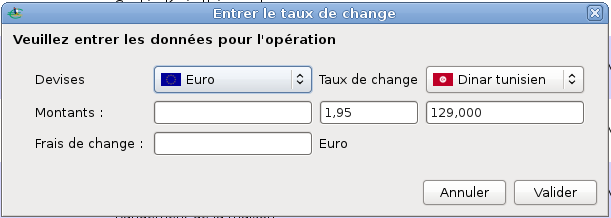
\includegraphics[scale=0.5]{image/screenshot/transactions_changeRate}
\end{center}
\caption{Frais et taux de change}
\label{transactions-changeRate-img}
\end{figure}
% image centrée 
\fi

\begin{itemize}
	 \item si vous n'avez pas créé de lien (taux de change) pour cette devise, Grisbi affiche la fenêtre de  \ifIllustration frais et taux de change \refimage{transactions-changeRate-img} :
	 \else frais et taux de change :
	 \fi
	  saisissez-y le taux de change, validez la fenêtre puis validez l'opération : le montant en devise s'affiche dans le champ \menu{Débit} et celui dans la devise du compte dans le champ \menu{Montant} ;
	  % espace pour notte alignée avec l'item
	  
	  \textbf{Note} : vous pouvez inverser le sens de la conversion (un euro vaut X Devise, ou bien une Devise vaut Y euros) en inversant le nom des devises dans les deux listes déroulantes ; vous pouvez ainsi entrer exactement le taux de change tel qu'il vous est communiqué ; ce taux peut être ajusté à tout moment après la création de l'opération.
	 \item si vous voulez modifier le taux de change, ouvrez l'opération en modification, cliquez sur le bouton \menu{Change} dans le formulaire de saisie, cochez la case de libellé \menu{Modifier le taux de change} si elle ne l'est pas, puis modifiez-le, et validez la fenêtre puis l'opération ;
	 \item si vous avez des \indexword{frais de change}\index{frais de change}, ouvrez l'opération en modification, cliquez sur le bouton \menu{Change} dans le formulaire de saisie, saisissez les frais en devise du compte dans le champ \menu{Frais de change}, et validez la fenêtre puis l'opération ; ces frais sont alors ajoutés au contenu du champ \menu{Montant} ; mais vous pouvez à la place les saisir dans une opération indépendante, en utilisant une catégorie dédiée, par exemple \emph{Frais financiers : Frais bancaires} : cela peut vous permettre de les comptabiliser à part ;
	 \item si vous voulez que le taux de change soit fixe : voir la section \vref{setup-resources-rate}, \menu{Liens entre devises}.
\end{itemize}


\section{Saisie d'une opération avec tiers virtuel\label{transactions-virtualThird}}


Grisbi vous permet d'utiliser des tiers virtuels : un tiers virtuel est un \emph{état} qui représente une liste de plusieurs tiers.

Lorsque vous saisissez une opération avec pour tiers un tiers virtuel, Grisbi enregistre, au moment de sa validation, une opération identique (montant, catégorie, imputation budgétaire, moyen de paiement etc.) pour \emph{chacun} des tiers représentés par ce tiers virtuel. Par exemple, vous pouvez saisir en une seule fois un appel à cotisation pour 200 adhérents d'une association, ce qui représente un gain de temps très appréciable\ldots

% espace pour changement de thème
\vspacepdf{5mm}
Pour \indexword{saisir une opération avec un tiers virtuel}\index{tiers virtuel !saisie d'opération}, saisissez ce tiers  dans le champ \menu{Tiers} du formulaire de saisie, sous la forme \og État : nom\_du\_tiers\_virtuel\fg{}. 

% espace pour changement de thème
\vspacepdf{5mm}
Pour créer un tiers virtuel, créez un état contenant une liste de tiers : voir le paragraphe \vref{reportscreation-display-general-virtualThird}, \menu{Tiers virtuel}.

% espace pour changement de thème
\vspacepdf{5mm}
Pour modifier un tiers virtuel, modifiez l'état qui l'a créé : voir la section \vref{reports-modify}, \menu{Modification d'un état}.

%espace pour changement de thème
\vspacepdf{5mm}
Pour supprimer un tiers virtuel, vous avez deux possibilités :

\begin{itemize}
	\item décochez la case \menu{Considérer les tiers de ce rapport comme un tiers virtuel} dans l'état qui le définit, puis validez (voir la section \vref{reports-modify}, \menu{Modification d'un état}) ;
	\item supprimez l'état qui le définit (voir la section \vref{reports-delete}, \menu{Suppression d'un état}).
\end{itemize}

\ifIllustration
% saut de page pour titre solidaire
\newpage
\fi


\section{Ventilation d'une opération\label{transactions-breakdown}}


\indexword{Ventiler une opération}\index{ventiler !opération} signifie répartir son montant entre plusieurs lignes (par exemple, vos achats au supermarché peuvent se répartir entre les catégories \emph{Alimentation} et \emph{Soins : Habillement}). Vous pouvez aussi répartir une somme sur la même catégorie, mais avec des informations différentes dans le champ \menu{Remarques} (par exemple pour mémoriser le détail d'une opération).


\subsection{Saisie de l'opération ventilée\label{transactions-breakdown-master}}

Pour \indexword{saisir une opération ventilée}\index{opération !ventilée}, procédez comme suit :
	 
\begin{enumerate}
	 \item dans le formulaire, commencez la saisie de votre opération comme une opération normale jusqu'au champ \menu{Catégories}, où vous choisissez la catégorie \menu{Opération ventilée} (vers la fin du menu déroulant, mais il est plus simple de taper \og O \fg{}) ;
	 \item continuez à saisir les autres données, puis validez :
	 \item dans la liste des opérations, apparaissent la première ligne de la nouvelle opération en caractères rouges sur fond bleu{\couleur}, et en-dessous une nouvelle ligne, sur fond rouge{\couleur} donc sélectionnée, avec un total égal à zéro et un  écart égal à la différence entre ce total et la valeur totale de l'opération ventilée, donc \ifIllustration en négatif\refimage{transactions-breakdown-img} ;
	\else en négatif ;
	\fi
	
	\ifIllustration
	% image centrée 
	\begin{figure}[htbp]
	\begin{center}
	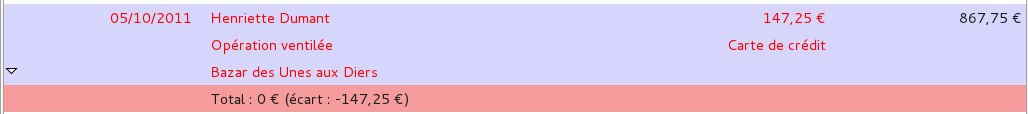
\includegraphics[scale=0.5]{image/screenshot/transactions_breakdown}
	\end{center}
	\caption{Saisie de l'opération ventilée}
	\label{transactions-breakdown-img}
	\end{figure}
	% image centrée 
	\fi

	 \item dans le formulaire, le curseur est dans le champ \menu{Débit}, et les champs  \menu{Date}, \menu{Tiers} et \menu{Moyen de paiement} sont grisés, ce qui signifie qu'on ne peut plus les modifier : il s'agit du formulaire de sous-opération, qui est prêt pour la saisie des sous-opérations ;
	 \item passez à la sous-section suivante \menu{Saisie des sous-opérations ventilées}.
\end{enumerate}


\subsection{Saisie des sous-opérations ventilées\label{transactions-breakdown-slave}}

Pour saisir les \indexword{sous-opérations ventilées}\index{sous-opération !ventilée}, continuez la saisie comme suit :

\textbf{Note} : le montant d'une sous-opération peut-être le résultat d'une opération portant sur plusieurs achats ou dépenses inscrites sur un ticket de caisse ou une facture ; vous pouvez donc utiliser la \indexword{calculatrice}\index{calculatrice} dans les champs de saisie \menu{Débit} ou \menu{Crédit} pour obtenir plus facilement les montants des sous-opérations (voir la section \vref{transactions-new-numbers}, \menu{Saisie de formules}).

\begin{enumerate}
	 \item dans ce formulaire de sous-opération, saisissez les champs libres (non grisés), puis validez votre première sous-opération ;
	 \item dans la liste des opérations, cette sous-opération s'affiche sur fond rose{\couleur}, et une nouvelle ligne apparaît, sur fond rouge{\couleur} donc sélectionnée, qui affiche un total égal à la première sous-opération saisie, en négatif, et un écart égal à la différence entre la valeur totale de l'opération ventilée et la valeur de cette sous-opération, \ifIllustration en négatif\refimage{transactions-breakdown-sub1-img} ;
	\else en négatif ;
	\fi
	
	\ifIllustration
	% image centrée 
	\begin{figure}[htp]
	\begin{center}
	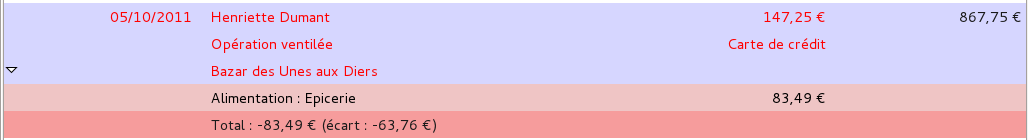
\includegraphics[scale=0.5]{image/screenshot/transactions_breakdown_sub1}
	\end{center}
	\caption{Saisie de la première sous-opération ventilée}
	\label{transactions-breakdown-sub1-img}
	\end{figure}
	% image centrée 
	\fi

	 \item il y a au moins deux sous-opérations dans une opération ventilée (sinon cela n'a aucun intérêt\ldots) ; donc, dans le formulaire de sous-opération, saisissez une deuxième sous-opération de la même manière, puis validez : cette sous-opération s'affiche sur fond rose{\couleur} et une nouvelle ligne apparaît, sur fond rouge{\couleur} donc sélectionnée, qui affiche le dernier total des sous-opérations saisies et le \ifIllustration dernier écart \refimage{transactions-breakdown-sub2-img} ;
	\else dernier écart ;
	\fi
	le total des sous-opérations a augmenté (en négatif) du montant de cette deuxième sous-opération, tandis que l'écart a diminué (en négatif) du même montant ; 

	\ifIllustration
	% image centrée 
	\begin{figure}[htp]
	\begin{center}
	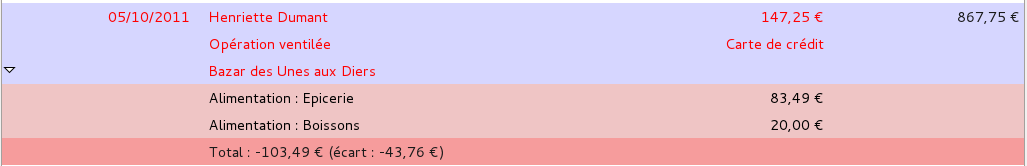
\includegraphics[scale=0.5]{image/screenshot/transactions_breakdown_sub2}
	\end{center}
	\caption{Saisie de la deuxième sous-opération ventilée}
	\label{transactions-breakdown-sub2-img}
	\end{figure}
	% image centrée 
	\fi

	 \item  si l'écart n'est pas nul, on peut alors saisir une troisième sous-opération de la \ifIllustration même manière\refimage{transactions-breakdown-sub3-img},
	\else même manière,
	\fi
	\ifIllustration
	% image centrée 
	\begin{figure}[htp]
	\begin{center}
	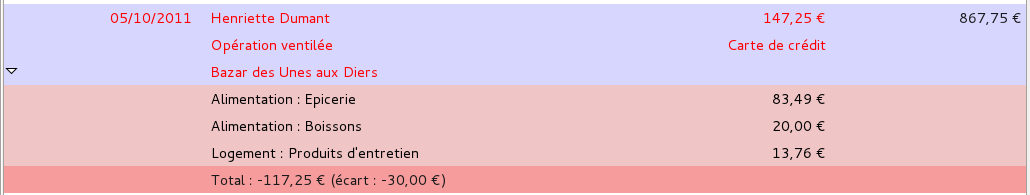
\includegraphics[scale=0.5]{image/screenshot/transactions_breakdown_sub3}
	\end{center}
	\caption{Saisie de la troisième sous-opération ventilée}
	\label{transactions-breakdown-sub3-img}
	\end{figure}
	% image centrée 
	\fi
	et ainsi de suite jusqu'à ce que le montant de votre dernière sous-opération soit exactement égal à l'écart affiché ; validez celle-ci : la dernière sous-opération s'affiche sur fond rose{\couleur} et une nouvelle ligne sur fond rose{\couleur} apparaît, vide, ce qui indique qu'il n'y a plus d'écart et que la somme des sous-opérations est bien égale à la valeur totale de l'opération \ifIllustration  ventilée\refimage{transactions-breakdown-complete-img}.
	\else ventilée.
	\fi
	
	\ifIllustration
	% image centrée 
	\begin{figure}[htp]
	\begin{center}
	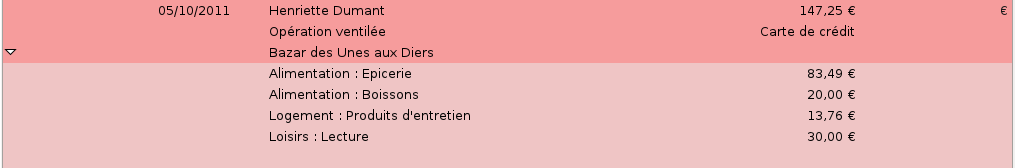
\includegraphics[scale=0.5]{image/screenshot/transactions_breakdown_complete}
	\end{center}
	\caption{Saisie de la dernière sous-opération ventilée}
	\label{transactions-breakdown-complete-img}
	\end{figure}
	% image centrée 
	\fi
	 
		 \item passez à la sous-section suivante \menu{Validation de l'opération ventilée}.
\end{enumerate}


\subsection{Validation de l'opération ventilée\label{transactions-breakdown-validation}}

À ce moment, toutes les sous-opérations sont entrées et validées et, dans la liste des opérations, la ligne de l'opération ventilée est affichée sur fond rouge{\couleur}, donc sélectionnée. Le formulaire réaffiche les données que vous y avez saisies. Toutes les sous-opérations étant correctes, validez l'opération ventilée, qui s'affiche alors dans la liste des opérations, en caractères noirs et sur fond rouge{\couleur}, sans les \ifIllustration sous-opérations\refimage{transactions-breakdown-oneLine-img}.
\else sous-opérations.
\fi

\ifIllustration
% image centrée 
\begin{figure}[htp]
\begin{center}
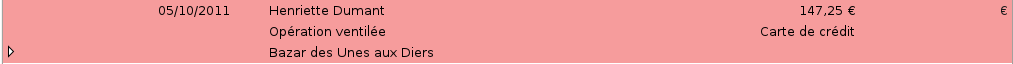
\includegraphics[scale=0.5]{image/screenshot/transactions_breakdown_oneLine}
\end{center}
\caption{Opération ventilée validée}
\label{transactions-breakdown-oneLine-img}
\end{figure}
% image centrée 
\fi

Une fois le dernier champ du formulaire saisi et validé, la ligne active, en rouge{\couleur}, passe à la dernière ligne vide de la liste, comme pour une opération normale.

Vous pouvez vérifier tout le contenu de cette opération ventilée, en cliquant sur le petit triangle à gauche de sa ligne pour dérouler \ifIllustration l'opération\refimage{transactions-breakdown-complete-img}. 
\else l'opération.
\fi

\textbf{Note} : ces triangles peuvent être remplacés, en fonction du thème de l'environnement de bureau ou du gestionnaire de fenêtres que vous utilisez, par d'autres caractères tels que +, -, >, <, etc.

% espace après Attention ou Note : 5 mm
\vspacepdf{5mm}
Vous pouvez alors modifier les sous-opérations en les sélectionnant et en modifiant leurs champs de la même manière, et de façon à ce que finalement leur somme soit égale à la valeur de l'opération ventilée.


\subsection{Rappel automatique d'une opération ventilée\label{transactions-breakdown-recall}}

Le \indexword{rappel automatique}\index{opération !rappel automatique} d'une opération ventilée 
fonctionne comme celui d'une opération normale (voir la section \vref{transactions-new-recall}, \menu{Rappel automatique d'une opération}). 

Cependant, pour une opération ventilée, un champ supplémentaire \menu{Restaurer les sous-opérations} apparaît en bas du formulaire de saisie, à gauche des boutons \menu{Annuler} et \menu{Valider}, et vous pouvez cocher la case correspondante en cliquant dessus ou sur le champ, et selon votre besoin.


\section{Modification d'une opération\label{transactions-modify}}


Pour modifier une opération ou une sous-opération ventilée, sélectionnez-la pour qu'elle s'affiche dans le formulaire de saisie, puis passez en mode édition par l'une de ces méthodes :

\begin{itemize}
	 \item appuyez sur la touche du clavier \key{Entrée} ;
	 \item dans la barre de menus, sélectionnez \menu{Édition - Éditer l'opération} ;
	 \item dans la barre d'outils, cliquez sur \menu{Éditer} ;
	 \item dans le menu contextuel, sélectionnez \menu{Éditer l'opération} ;
	 \item dans l'un des champs du formulaire, cliquez-gauche.
\end{itemize}
 
Si le formulaire de saisie n'était pas affiché, il s'affiche. La date s'affiche sur fond bleu{\couleur} dans le formulaire.

Il est alors possible de modifier toutes les informations désirées, en se déplaçant dans les champs de saisie. 

La combinaison de touches \key{Ctrl} \key{P} donne ou retire à une opération sélectionnée le statut d'\indexword{opération pointée}\index{opération !pointée}, et \key{Ctrl} \key{R} celui d'\indexword{opération rapprochée}\index{opération !rapprochée} (voir le chapitre \vref{reconciliation}, \menu{Rapprochement bancaire}). Vous pouvez aussi donner à une opération le statut d'opération pointée, mais uniquement celui-ci, par la combinaison \key{Ctrl} \key{Clic} dans la colonne P/R, sur la ligne de l'opération à pointer.

% espace pour changement de thème
\vspacepdf{5mm}
Si l'opération a déjà été rapprochée (voir le chapitre \vref{reconciliation}, \menu{Rapprochement bancaire}), il est par contre impossible de modifier son montant. Les autres champs restent modifiables. Si vous avez vraiment et impérativement besoin de modifier le montant (mais si vous avez déjà rapproché l'opération, cela ne devrait pas être le cas), procédez comme suit :

\begin{enumerate}
	 \item sélectionnez l'opération ;
	 \item annulez son statut \emph{Rapproché} en appuyant sur la combinaison de touches \key{Ctrl} \key{R} ;
	 \item modifiez l'opération ;
	 \item appuyez à nouveau sur la combinaison de touches \key{Ctrl} \key{R}. Si vous ne le faisiez pas, le rapprochement relatif à cette opération serait faussé, d'une valeur égale à la différence entre le précédent et le nouveau montant de cette opération.
\end{enumerate}

\strong{Attention} : cette manipulation est hautement déconseillée, car elle fausse momentanément le rapprochement associé à cette opération, et il redevient exact à la fin, si vous n'en avez pas modifié le montant (cette manipulation sera d'ailleurs probablement automatiquement désactivée dans une future version de Grisbi dans le cas d'une comptabilité de type association).


\section{Suppression d'une opération\label{transactions-delete}}


Pour supprimer une opération, sélectionnez-la, et utilisez l'une de ces
méthodes :
\begin{itemize}
	 \item appuyez sur la touche du clavier \key{Suppr} ;
	 \item dans la barre de menus, sélectionnez \menu{Édition - Supprimer une opération} ;
	 \item dans la barre d'outils, cliquez-gauche sur \menu{Supprimer} ;
	 \item dans le menu contextuel, sélectionnez \menu{Supprimer l'opération}.
\end{itemize}

% espace pour changement de thème
\vspacepdf{5mm}
La suppression d'une sous-opération ventilée se fait de la même façon, mais vous devrez faire en sorte que finalement la somme des sous-opérations soit égale à la valeur de l'opération ventilée.

\ifIllustration
% espace pour changement de thème
\vspacepdf{5mm}
\fi

La suppression n'est pas possible si :

\begin{itemize}
	 \item l'opération est ouverte en modification : il faut préalablement sortir du mode édition, en utilisant la touche \key{Échap} ;
	 \item l'opération est \indexword{rapprochée}\index{opération !rapprochée} (il faut préalablement annuler son statut \emph{Rapproché} en appuyant sur la combinaison de touches \key{Ctrl} \key{R}).
\end{itemize}

% espace avant Attention ou Note  : 5 mm
\vspacepdf{5mm}
\strong{Attention} : cette dernière manipulation est hautement déconseillée car elle fausse le rapprochement associé à cette opération.


\section{Opération sélectionnée comme modèle\label{transactions-model}}


Pour utiliser une \indexword{opération comme modèle}\index{opération !modèle}, sélectionnez-la, et utilisez l'une de ces méthodes :
\begin{itemize}
	 \item dans la barre de menus, sélectionnez \menu{Édition - Utiliser l'opération sélectionnée comme modèle} ;
	 \item dans le menu contextuel, sélectionnez \menu{Édition - Utiliser l'opération sélectionnée comme modèle}.
\end{itemize}

% espace pour changement de thème
\vspacepdf{5mm}
Une nouvelle opération s'affiche sur fond rouge{\couleur}, dans une nouvelle ligne en-dessous de l'opération sélectionnée précédemment ; elle n'a évidemment ni le statut \emph{Pointé} ni le statut \emph{Rapproché}.

Vous pouvez alors éditer cette nouvelle opération, par exemple en modifiant sa date.


\section{Clonage d'une opération\label{transactions-duplicate}}


Pour cloner une opération, sélectionnez-la pour qu'elle s'affiche dans le formulaire de saisie, puis utilisez l'une de ces deux méthodes :

\begin{itemize}
	 \item dans la barre de menus, sélectionnez \menu{Édition - Cloner l'opération} ;
	 \item dans le menu contextuel, sélectionnez \menu{Cloner l'opération}.
\end{itemize}

% espace pour changement de thème
\vspacepdf{5mm}
L'opération sélectionnée précédemment apparaît toujours sur fond rouge{\couleur}, et l'opération clonée s'affiche dans une nouvelle ligne en-dessous ; elle n'a évidemment ni le statut \emph{Pointé} ni le statut \emph{Rapproché}.

Vous pouvez alors éditer cette nouvelle opération, par exemple en modifiant la date.


\section{Conversion d'une opération en opération planifiée\label{transactions-schedule}}


Pour convertir une opération en opération planifiée, sélectionnez-la pour qu'elle s'affiche dans le formulaire de saisie, puis utilisez l'une de ces deux méthodes :
\begin{itemize}
	 \item dans la barre de menus, sélectionnez \menu{Édition - Convertir en opération planifiée} ;
	 \item dans le menu contextuel, sélectionnez \menu{Convertir l'opération en opération planifiée}.
\end{itemize}

% espace pour changement de thème
\vspacepdf{5mm}
L'onglet \menu{Échéancier} s'affiche. La nouvelle opération apparaît dans la liste des opérations planifiées, et le formulaire de saisie s'affiche avec les paramètres de l'opération. Vérifiez ou éditez ces paramètres selon vos besoins, puis validez.


\section{Déplacement d'une opération vers un autre compte\label{transactions-move}}


Pour déplacer une opération dans un autre compte, sélectionnez-la, puis utilisez l'une de ces deux méthodes :

\begin{itemize}
	 \item dans la barre de menus, sélectionnez \menu{Édition - Déplacer l'opération vers un autre compte} et choisissez le compte destinataire dans la liste ;
	 \item dans le menu contextuel, sélectionnez \menu{Déplacer l'opération vers un autre compte} et choisissez le compte destinataire dans la liste.
\end{itemize}

Il est bien entendu que les deux comptes doivent se trouver dans le même fichier de comptes.

% espace avant Attention ou Note  : 5 mm
\vspacepdf{5mm}
\textbf{Note} : il est impossible de déplacer une opération si elle a le statut \emph{Rapproché}. Par contre, c'est possible si elle a le statut \emph{Pointé}.


\section{Nouveau tiers, catégorie ou imputation budgétaire\label{transactions-fillcombo}}


Il peut arriver que vous ayez besoin d'un nouveau tiers, d'une nouvelle catégorie ou d'une nouvelle imputation budgétaire pendant une saisie d'opération. Dans ce cas, Grisbi permet d'en faire la création \og à la volée \fg{} : saisissez le nouveau nom dans la zone de liste déroulante, et Grisbi l'ajoutera automatiquement à la liste. Vous pourrez ultérieurement faire toutes les modifications nécessaires dans les onglets \menu{Tiers} (voir la section \vref{thirdparties-modify}, \menu{Modification d'un tiers}), \menu{Catégories} (voir la section \vref{categories-modify}, \menu{Modification d'une catégorie ou d'une sous-catégorie}) ou \menu{Imputations budgétaires} (voir la section \vref{budgetarylines-modify}, \menu{Modification d'une (sous-) imputation budgétaire}).
 
% espace avant Attention ou Note  : 5 mm
\vspacepdf{5mm} 
\textbf{Note} : pour saisir une \indexword{catégorie}\index{catégories !syntaxe}\index{sous-catégories !syntaxe}\index{syntaxe !catégories : sous-catégories}
 (ou une \indexword{imputation budgétaire} : sous-imputation budgétaire\index{imputations budgétaires !syntaxe}\index{sous-imputations budgétaires !syntaxe}\index{syntaxe !imputations budgétaires : sous-imputations budgétaires}) avec une sous-catégorie (ou sous-imputation), il faut respecter la syntaxe \emph{catégorie : sous-catégorie} (avec les deux points comme séparateur, encadrés par des espaces), sinon Grisbi ne comprendra pas. De même si vous ajoutez une nouvelle sous-catégorie (ou sous-imputation budgétaire) à une catégorie (ou imputation) existante.
% espace après Attention ou Note  : 5 mm
\vspacepdf{5mm}

Vous pouvez également créer un tiers, une catégorie ou une imputation budgétaire directement dans leur onglet respectif, sélectionné dans le panneau de navigation.


\section{Impression de la liste des opérations\label{transactions-print}}


Pour imprimer la liste des opérations, cliquez sur le bouton \menu{Imprimer} de la barre d'outils ; une fenêtre d'impression s'ouvre, dont l'aspect et les fonctions dépendent de votre gestionnaire d'impression ; vous aurez le plus souvent les choix suivants :

\begin{itemize}
	\item imprimer dans un fichier (au format \gls{PostScript}, \gls{PDF} ou \gls{SVG}) ;
	\item imprimer avec votre imprimante.
\end{itemize}

En fonction de votre gestionnaire d'impression, vous pourrez disposer de réglages divers tels que la taille et l'orientation de la feuille, la résolution, la police d'impression et sa taille, etc.

% espace avant Attention ou Note  : 5 mm
\vspacepdf{5mm}
\textbf{Note} : la liste des opérations de certains comptes peut être très longue ; affichez un aperçu avant impression pour vérifier ce que vous allez imprimer.


%XXXXXXXXXXXXXXXXXXXXXXXXXXXXXXXXXXXXXXXXXXXXXXXXXXXXXXXXXXXXXXXXXXXXXXXXXXXXXXXXXX
%
% [benj] supprimé car franchement, ça n'a rien à faire ici.
%
% PLEASE NOTE !  DO NOT TRANSLATE THE FOLLOWING SECTION
%\section{Quelques mots sur un anglicisme trop répandu}
%
%On voit régulièrement dans les documentations, livres et autres articles,
%publiés sur l'Internet et ailleurs, le mot \emph{complétion}. Ceci est un
%horrible anglicisme. 
%
%Que l'on assimile un mot anglais lorsque le mot français équivalent n'existe pas
%peut se comprendre, encore que le néologisme intelligent me semble préférable.
%Il ne s'agit bien sûr pas de tomber dans le ridicule de nos académiciens qui
%traduisent mail par mèl et CD-Rom par cédérom. Passons sur leur manque
%d'imagination alors qu'ils ont su par autrefois créer des mots comme disquette,
%informatique et ordinateur, qui n'existent nulle part ailleurs !
%
%Dans le cas précis du mot \emph{complétion} un traducteur du \emph{Guide de
%l'administration réseau sous linux,} Editions O'Reilly, avait cru bien faire en
%essayant de créer le mot \emph{complétement} (avec un accent aigu) qui voulait
%signifier \emph{action de compléter}. L'initiative était louable mais ô combien
%risquée \ldots En effet lorsque l'on s'essaye à ce genre d'exercice de style, il est
%prudent de maîtriser tous les rouages de la langue. Et en l'occurrence il existe
%une règle dite la \emph{règle de l'ernance} (page 56 du \emph{Bescherelle
%Orthographe}) \footnote{Si quelqu'un possède ce livre je serais très heureux
%qu'il me fasse parvenir le texte exact de cette règle. Je ne l'ai 
%malheureusement plus\ldots} qui explique parfaitement le mécanisme de
%changement d'accent entre un verbe et le substantif dérivé
%\footm{André Cianfarini, qui se définit lui-même comme \emph{un développeur autodidacte qui n'a jamais fini sa thèse de grammaire pour cause de relations passionnelles avec l'informatique} me communique les précisions suivantes : 
%\begin{quote}
%C'est un processus phonologique qui est à l'origine de ces
%transformations ; pour simplifier, on pourrait le résumer ainsi :
%un "e" fermé (l'avant-dernier "e" de "préférer" par exemple) devient un
%"e" ouvert (l'avant-dernier "e" de "je préfère" par exemple) lorsque la
%syllabe qui le suit est atone.
%\end{quote} 
%}. Si ce malheureux
%traducteur l'avait connue il n'aurait pas commis cet affreux barbarisme\ldots
%
%Et si avant toute chose ce traducteur avait eu l'idée de vérifier dans son
%dictionnaire que le mot n'existait pas déjà\ldots il aurait trouvé :
%
%\begin{description}
%
%\item [complètement]n.m. Action de compléter : \emph{le complètement
%d'un livre}. 
%
%\end{description}
%
%Et j'ai bien pris soin de chercher ce mot dans le plus vieil exemplaire du
%\emph{Larousse universel} en ma possession, soit l'édition de 1949 !
%
%Donc adoptons sans aucun remord le mot complètement, et, puisque cette action
%est automatique, allons sans crainte jusqu'à écrire auto-complètement, ce qui
%est parfaitement compréhensible, intuitif et 100\% français !
%
%Cocorico !
%
%Et puissent ces quelques lignes tordre définitivement le cou au mot complétion,
%cette \emph{affreuseté non-permissable} ! ;-)
%
%from now you can translate again